\documentclass[a4paper,12pt]{extarticle}
\usepackage[utf8x]{inputenc}
\usepackage[T1,T2A]{fontenc}
\usepackage[russian]{babel}
\usepackage[hidelinks]{hyperref}
\usepackage{indentfirst}
\usepackage{listings}
\usepackage{color}
\usepackage{here}
\usepackage{array}
\usepackage{multirow}
\usepackage{graphicx}
\usepackage{subcaption} 
\usepackage{mathtools}

\usepackage{caption}
\renewcommand{\lstlistingname}{Программа} % заголовок листингов кода

\bibliographystyle{ugost2008ls}

\usepackage{listings}
\lstset{ %
extendedchars=\true,
keepspaces=true,
language=C,						% choose the language of the code
basicstyle=\footnotesize,		% the size of the fonts that are used for the code
numbers=left,					% where to put the line-numbers
numberstyle=\footnotesize,		% the size of the fonts that are used for the line-numbers
stepnumber=1,					% the step between two line-numbers. If it is 1 each line will be numbered
numbersep=5pt,					% how far the line-numbers are from the code
backgroundcolor=\color{white},	% choose the background color. You must add \usepackage{color}
showspaces=false				% show spaces adding particular underscores
showstringspaces=false,			% underline spaces within strings
showtabs=false,					% show tabs within strings adding particular underscores
frame=single,           		% adds a frame around the code
tabsize=2,						% sets default tabsize to 2 spaces
captionpos=t,					% sets the caption-position to top
breaklines=true,				% sets automatic line breaking
breakatwhitespace=false,		% sets if automatic breaks should only happen at whitespace
escapeinside={\%*}{*)},			% if you want to add a comment within your code
postbreak=\raisebox{0ex}[0ex][0ex]{\ensuremath{\color{red}\hookrightarrow\space}},
texcl=true,
inputpath=listings,                     % директория с листингами
}

\usepackage[left=2cm,right=2cm,
top=2cm,bottom=2cm,bindingoffset=0cm]{geometry}

%% Нумерация картинок по секциям
\usepackage{chngcntr}
\counterwithin{figure}{section}
\counterwithin{table}{section}

%%Точки нумерации заголовков
\usepackage{titlesec}
\titlelabel{\thetitle.\quad}
\usepackage[dotinlabels]{titletoc}

%% Оформления подписи рисунка
\addto\captionsrussian{\renewcommand{\figurename}{Рисунок}}
\captionsetup[figure]{labelsep = period}

%% Подпись таблицы
%\DeclareCaptionFormat{hfillstart}{\hfill#1#2#3\par}
%\captionsetup[table]{format=hfillstart,labelsep=newline,justification=centering,skip=-10pt,textfont=bf}

%% Путь к каталогу с рисунками
\graphicspath{{fig/}}

%% Внесение titlepage в учёт счётчика страниц
\makeatletter
\renewenvironment{titlepage} {
 \thispagestyle{empty}
}
\makeatother

\DeclarePairedDelimiter\abs{\lvert}{\rvert}%
\DeclarePairedDelimiter\norm{\lVert}{\rVert}%

\usepackage{amsmath}

\begin{document}	% начало документа

% Титульная страница
\begin{titlepage}	% начало титульной страницы

	\begin{center}		% выравнивание по центру

		\large Санкт-Петербургский политехнический университет Петра Великого\\
		\large Институт прикладной математики и механики \\
		\large Кафедра <<Прикладная математика>>\\[6cm]
		% название института, затем отступ 6см
		
		\huge Математическая статистика\\[0.5cm] % название работы, затем отступ 0,5см
		%\huge Методы оптимизации\\[0.5cm] % название работы, затем отступ 0,5см
		\large \textbf{Отчет по лабораторной работе №4}\\[5.1cm]
		%\large \textbf{Отчет по лабораторной работе \\``Решение задач одномерной минимизации ``}\\[5.1cm]
		%\\[5cm]

	\end{center}


	\begin{flushright} % выравнивание по правому краю
		\begin{minipage}{0.25\textwidth} % врезка в половину ширины текста
			\begin{flushleft} % выровнять её содержимое по левому краю

				\large\textbf{Работу выполнил:}\\
				\large Колесник В.Н.\\
				\large {Группа:} 3630102/70201\\
				
				\large \textbf{Преподаватель:}\\
				\large к.ф.-м.н., доцент\\
				\large Баженов Александр Николаевич
				%\large Родионова Елена Александровна

			\end{flushleft}
		\end{minipage}
	\end{flushright}
	
	\vfill % заполнить всё доступное ниже пространство

	\begin{center}
	\large Санкт-Петербург\\
	\large \the\year % вывести дату
	\end{center} % закончить выравнивание по центру

\end{titlepage} % конец титульной страницы

\vfill % заполнить всё доступное ниже пространство


% Содержание
\renewcommand\contentsname{\centerline{Содержание}}
\tableofcontents
\newpage

\listoffigures
\newpage

\listoftables
\newpage

\section{Постановка задачи}
Сгенерировать двумерные выборки размерами 20, 60, 100 для нормального двумерного распределения $N(x, y, 0, 0, 1, 1, \rho)$.\\
Коэффициент корреляции $\rho$ взять равным 0, 0.5, 0.9.\\
Каждая выборка генерируется 1000 раз и для неё вычисляются: среднее значение, среднее значение квадрата и дисперсия коэффициентов корреляции Пирсона, Спирмена и квадрантного коэффициента корреляции.\\
Повторить все вычисления для смеси нормальных распределений:
\begin{equation} \label{func}
f(x, y) = 0.9N(x, y, 0, 0, 1, 1, 0.9) + 0.1N(x, y, 0, 0, 10, 10,−0.9).
\end{equation}
Изобразить сгенерированные точки на плоскости и нарисовать эллипс равновероятности.

\section{Теория}
\subsection{Двумерное нормальное распределение}
Двумерная случайная величина ($X, Y$) называется распределённой нормально (или просто нормальной), если её плотность вероятности определена формулой
\begin{gather}
N(x, y, \overline{x}, \overline{y}, \sigma_x, \sigma_y, \rho)=\frac{1}{2\pi \sigma_x\sigma_y\sqrt{1-\rho^2}}\times \\
\times exp \{-\frac{1}{2(1-\rho^2)}[\frac{(x-\overline{x})^2}{\sigma_x^2}-2\rho\frac{(x-\overline{x})(y-\overline{y})}{\sigma_x \sigma_y}+\frac{(y-\overline{y})^2}{\sigma_y^2}]\}
\end{gather}
Компоненты $X, Y$ двумерной нормальной случайной величины также распределены нормально с математическими ожиданиями $x, y$ и средними квадратическими отклонениями $\sigma_x, \sigma_y$ соответственно.
Параметр $\rho$ называется коэффициентом корреляции.

\subsection{Корреляционный момент (ковариация) и коэффи-
циент корреляции}
Корреляционным моментом, иначе ковариацией, двух случайных величин $X$ и $Y$ называется математическое ожидание произведения отклонений этих случайных величин от их математических ожиданий.
\begin{equation}
K=cov(X,Y)=M[(X-\overline{x})(Y-\overline{y})]
\end{equation}
Коэффициентом корреляции $\rho$ двух случайных величин $X$ и $Y$ называется отношение их корреляционного момента к произведению их средних квадратических отклонений:
\begin{equation}
\rho=\frac{K}{\sigma_x \sigma_y}
\end{equation}
Коэффициент корреляции — это нормированная числовая характеристика, являющаяся мерой близости зависимости между случайными величинами к линейной.

\subsection{Выборочные коэффициенты корреляции}
\subsubsection{Выборочный коэффициент корреляции Пирсона}
Пусть по выборке значений $\{x_i,y_i\}_1^n$ двумерной с.в. $(X,Y)$ требуется оценить коэффициент корреляции $\rho=\frac{cov(X,Y)}{\sqrt{DX DY}}$. Естественной оценкой для $\rho$ служит его статистический аналог в виде выборочного коэффициента корреляции, предложенного К.Пирсоном, —
\begin{equation}
r=\frac{\frac{1}{n}\Sigma (x_i-\overline{x})(y_i-\overline{y})}{\sqrt{\frac{1}{n}\Sigma (x_i-\overline{x})^2 \frac{1}{n}\Sigma (y_i-\overline{y})^2}}=\frac{K}{s_X s_Y}
\end{equation}
где $K,s_X^2,s_Y^2$ — выборочные ковариация и дисперсии с.в. $X$ и $Y$.

\subsubsection{Выборочный квадрантный коэффициент корреляции}
Кроме выборочного коэффициента корреляции Пирсона, существуют и другие оценки степени взаимосвязи между случайными величинами. К ним относится выборочный квадрантный коэффициент корреляции
\begin{equation}
r_Q=\frac{(n_1+n_3)-(n_2+n_4)}{n},
\end{equation}
где $n_1, n_2, n_3$ и $n_4$ — количества точке с координатами $(x_i, y_i)$, попавшими соответственно в I, II, III и IV квадранты декартовой системы с осями $x'=x-med x, y'=y-med y$ и с центром в точке с координатами $(med x, med y)$.

\subsubsection{Выборочный коэффициент ранговой корреляции Спирмена}
На практике нередко требуется оценить степень взаимодействия между качественными признаками изучаемого объекта. Качественным называется признак, который нельзя измерить точно, но который позволяет сравнивать изучаемые объекты между собой и располагать их в порядке убывания или возрастания их качества. Для этого объекты выстраиваются в определённом порядке в соответствии с рассматриваемым признаком. Процесс упорядочения называется ранжированием, и каждому члену упорядоченной последовательности объектов присваивается ранг, или порядковый номер. Например, объекту с наименьшим значением признака присваивается ранг 1, следующему за ним объекту — ранг 2, и т.д. Таким образом, происходит сравнение каждого объекта со всеми объектами изучаемой выборки.\\
Если объект обладает не одним, а двумя качественными признаками — переменными $X$ и $Y$, то для исследования их взаимосвязи используют выборочный коэффициент корреляции между двумя последовательностями рангов этих признаков.\\
Обозначим ранги, соотвествующие значениям переменной $X$, через $u$, а ранги, соотвествующие значениям переменной $Y$, — через $v$.\\
Выборочный коэффициент ранговой корреляции Спирмена определяется как выборочный коэффициент корреляции Пирсона между рангами $u, v$ переменных $X, Y$:
\begin{equation}
r_S=\frac{\frac{1}{n}\Sigma (u_i-\overline{u})(v_i-\overline{v})}{\sqrt{\frac{1}{n}\Sigma (u_i-\overline{u})^2 \frac{1}{n}\Sigma (v_i-\overline{v})^2}}=\frac{K}{s_X s_Y}
\end{equation}
где $\overline{u}=\overline{v}=\frac{1+2+...+n}{n}=\frac{n+1}{2}$ - среднее значение рангов.

\subsubsection{Эллипсы рассеивания}
Рассмотрим поверхность распределения, изображающую функцию (\ref{func}). Она имеет вид холма, вершина которого находится над точкой $(x, y)$.\\
В сечении поверхности распределения плоскостями, параллельными оси $N(x, y, \overline{x}, \overline{y}, \sigma_x, \sigma_y, \rho)$, получаются кривые, подобные нормальным кривым распределения. В сечении поверхности распределения плоскостями, параллельными плоскости $xOy$, получаются эллипсы. Напишем уравнение проекции такого эллипса на плоскость $xOy$:
\begin{equation}
\frac{(x-\overline{x})^2}{\sigma_x^2}-2\rho\frac{(x-\overline{x})(y-\overline{y})}{\sigma_x \sigma_y}+\frac{(y-\overline{y})^2}{\sigma_y^2}=const
\end{equation}
Уравнение эллипса можно проанализировать обычными методами аналитической геометрии. Применяя их, убеждаемся, что центр эллипса находится в точке с координатами $(x, y)$; что касается направления осей симметрии эллипса, то они составляют с осью $Ox$ углы, определяемые уравнением
\begin{equation}
tg 2\alpha=\frac{2\rho \sigma_x \sigma_y}{\sigma_x^2-\sigma_y^2}.
\end{equation}
Это уравнение дает два значения углов: $\alpha$ и $\alpha_1$, различающиеся на $\frac{\pi}{2}$.\\
Таким образом, ориентация эллипса относительно координатных осей находится в прямой зависимости от коэффициента корреляции $\rho$ системы $(X, Y)$; если величины не коррелированны (т.е. в данном случае и независимы), то оси симметрии эллипса параллельны координатным осям; в противном случае они составляют с координатными осями некоторый угол.\\
Пересекая поверхность распределения плоскостями, параллельными плоскости $xOy$, и проектируя сечения на плоскость $xOy$ мы получим целое семейство подобных и одинаково расположенных эллипсов с общим центром $(x, y)$. Во всех точках каждого из таких эллипсов плотность распределения $N(x, y, \overline{x}, \overline{y}, \sigma_x, \sigma_y, \rho)$ постоянна. Поэтому такие эллипсы называются эллипсами равной плотности или, короче эллипсами рассеивания. Общие оси всех эллипсов рассеивания называются главными осями рассеивания.

\section{Реализация}
Лабораторная работа выполнена с помощью встроенных средств языка программирования R в среде разработки RStudio. Исходный код лабораторной работы приведён в приложении.

\section{Результаты}
\subsection{Выборочные коэффициенты корреляции}
\newpage
\begin{table}[h]
	\centering
		\begin{tabular} {|c|c|c|c|}
			\hline
			$\rho=0$ & $r$ & $r_S$ & $r_Q$ \\ \hline
			$E(z)$ & -0.005 & -0.005 & -0.008 \\ \hline
			$E(z^2)$ & 0.057 & 0.056 & 0.050 \\ \hline
			$D(z)$ & 0.057 & 0.056 & 0.050 \\ \hline
			&&&\\ \hline
			$\rho=0.5$ & $r$ & $r_S$ & $r_Q$ \\ \hline
			$E(z)$ & 0.489 & 0.462 & 0.331 \\ \hline
			$E(z^2)$ & 0.270 & 0.249 & 0.156 \\ \hline
			$D(z)$ & 0.031 & 0.036 & 0.046 \\ \hline
			&&&\\ \hline
			$\rho=0.9$ & $r$ & $r_S$ & $r_Q$ \\ \hline
			$E(z)$ & 0.896 & 0.867 & 0.711 \\ \hline
			$E(z^2)$ & 0.805 & 0.756 & 0.529 \\ \hline
			$D(z)$ & 0.002 & 0.004 & 0.024 \\ \hline
		\end{tabular}
	\caption{Двумерное нормальное распределение, $n=20$}
\end{table}

\begin{table}[h]
	\centering
		\begin{tabular} {|c|c|c|c|}
			\hline
			$\rho=0$ & $r$ & $r_S$ & $r_Q$ \\ \hline
			$E(z)$ & -0.004 & -0.005 & -0.007 \\ \hline
			$E(z^2)$ & 0.017 & 0.017 & 0.016 \\ \hline
			$D(z)$ & 0.017 & 0.017 & 0.016 \\ \hline
			&&&\\ \hline
			$\rho=0.5$ & $r$ & $r_S$ & $r_Q$ \\ \hline
			$E(z)$ & 0.503 & 0.483 & 0.338 \\ \hline
			$E(z^2)$ & 0.262 & 0.244 & 0.128 \\ \hline
			$D(z)$ & 0.009 & 0.010 & 0.014 \\ \hline
			&&&\\ \hline
			$\rho=0.9$ & $r$ & $r_S$ & $r_Q$ \\ \hline
			$E(z)$ & 0.897 & 0.881 & 0.711 \\ \hline
			$E(z^2)$ & 0.806 & 0.777 & 0.513 \\ \hline
			$D(z)$ & 0.0006 & 0.001 & 0.008 \\ \hline
		\end{tabular}
	\caption{Двумерное нормальное распределение, $n=60$}
\end{table}

\begin{table}[h]
	\centering
		\begin{tabular} {|c|c|c|c|}
			\hline
			$\rho=0$ & $r$ & $r_S$ & $r_Q$ \\ \hline
			$E(z)$ & 0.004 & 0.004 & 0.004 \\ \hline
			$E(z^2)$ & 0.010 & 0.010 & 0.010 \\ \hline
			$D(z)$ & 0.010 & 0.010 & 0.010 \\ \hline
			&&&\\ \hline
			$\rho=0.5$ & $r$ & $r_S$ & $r_Q$ \\ \hline
			$E(z)$ & 0.493 & 0.473 & 0.329 \\ \hline
			$E(z^2)$ & 0.248 & 0.230 & 0.117 \\ \hline
			$D(z)$ & 0.006 & 0.006 & 0.008 \\ \hline
			&&&\\ \hline
			$\rho=0.9$ & $r$ & $r_S$ & $r_Q$ \\ \hline
			$E(z)$ & 0.898 & 0.885 & 0.710 \\ \hline
			$E(z^2)$ & 0.808 & 0.784 & 0.509 \\ \hline
			$D(z)$ & 0.0003 & 0.0006 & 0.004 \\ \hline
		\end{tabular}
	\caption{Двумерное нормальное распределение, $n=100$}
\end{table}

\begin{table}[h]
	\centering
		\begin{tabular} {|c|c|c|c|}
			\hline
			$n=20$ & $r$ & $r_S$ & $r_Q$ \\ \hline
			$E(z)$ & 0.785 & 0.753 & 0.592 \\ \hline
			$E(z^2)$ & 0.625 & 0.579 & 0.381 \\ \hline
			$D(z)$ & 0.008 & 0.011 & 0.030 \\ \hline
			&&&\\ \hline
			$n=60$ & $r$ & $r_S$ & $r_Q$ \\ \hline
			$E(z)$ & 0.787 & 0.766 & 0.580 \\ \hline
			$E(z^2)$ & 0.622 & 0.590 & 0.347 \\ \hline
			$D(z)$ & 0.002 & 0.003 & 0.010 \\ \hline
			&&&\\ \hline
			$n=100$ & $r$ & $r_S$ & $r_Q$ \\ \hline
			$E(z)$ & 0.790 & 0.771 & 0.579 \\ \hline
			$E(z^2)$ & 0.625 & 0.596 & 0.342 \\ \hline
			$D(z)$ & 0.001 & 0.001 & 0.006 \\ \hline
		\end{tabular}
	\caption{Смесь нормальных распределений}
\end{table}

\newpage
\subsection{Эллипсы рассеивания}
\begin{figure}[!htb]
    \centering
    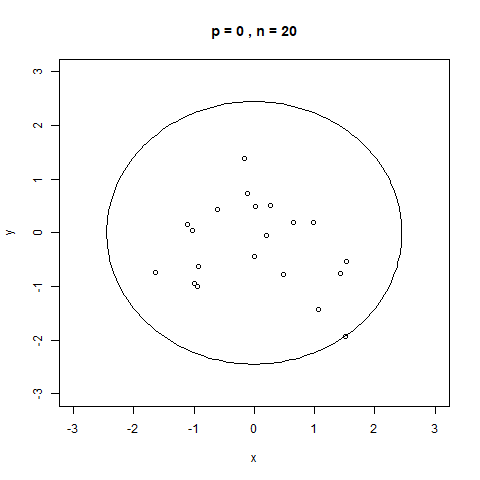
\includegraphics[width=0.3\textwidth]{20_0}
    \caption{$\rho=0, n=20$}
\end{figure}
\newpage
\begin{figure}[!htb]
    \centering
    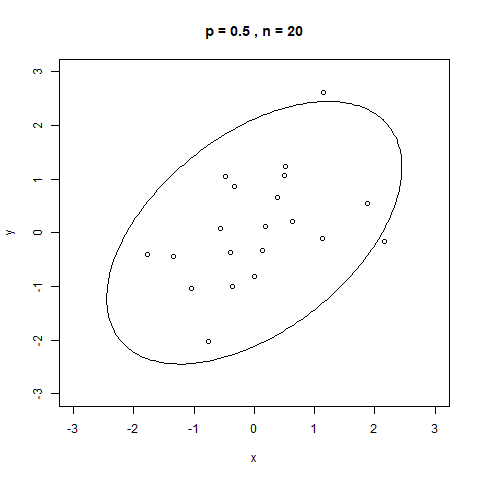
\includegraphics[width=0.3\textwidth]{20_0.5}
    \caption{$\rho=0.5, n=20$}
\end{figure}

\begin{figure}[!htb]
    \centering
    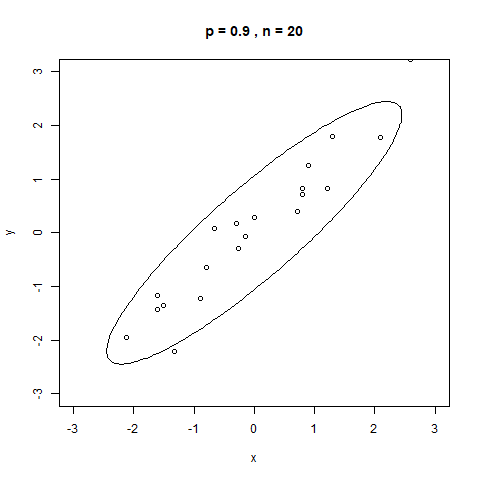
\includegraphics[width=0.3\textwidth]{20_0.9}
    \caption{$\rho=0.9, n=20$}
\end{figure}

\begin{figure}[!htb]
    \centering
    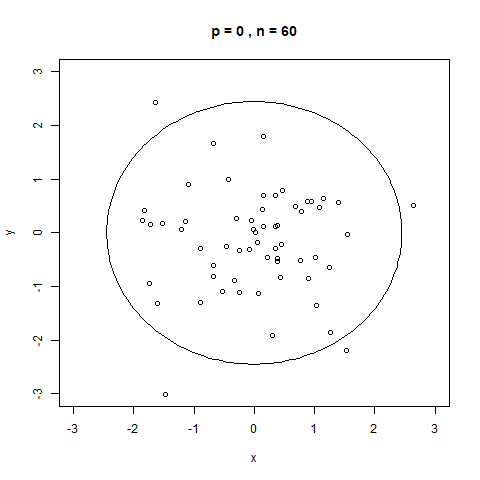
\includegraphics[width=0.3\textwidth]{60_0}
    \caption{$\rho=0, n=60$}
\end{figure}

\begin{figure}[!htb]
    \centering
    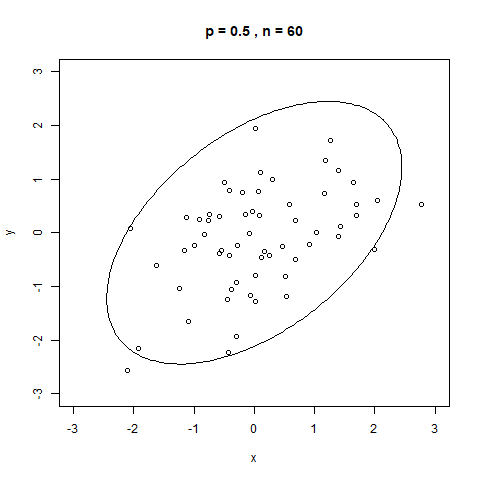
\includegraphics[width=0.3\textwidth]{60_0.5}
    \caption{$\rho=0.5, n=60$}
\end{figure}
\newpage
\begin{figure}[!htb]
    \centering
    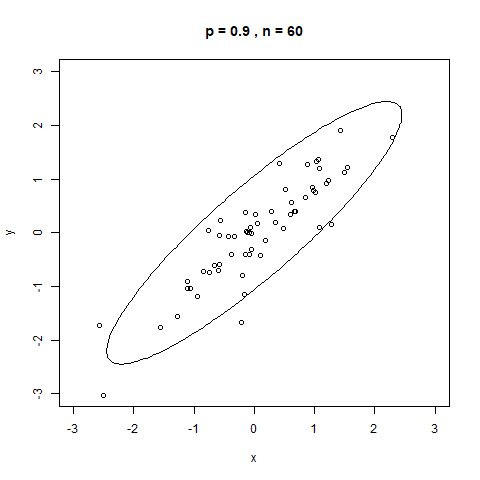
\includegraphics[width=0.3\textwidth]{60_0.9}
    \caption{$\rho=0.9, n=60$}
\end{figure}

\begin{figure}[!htb]
    \centering
    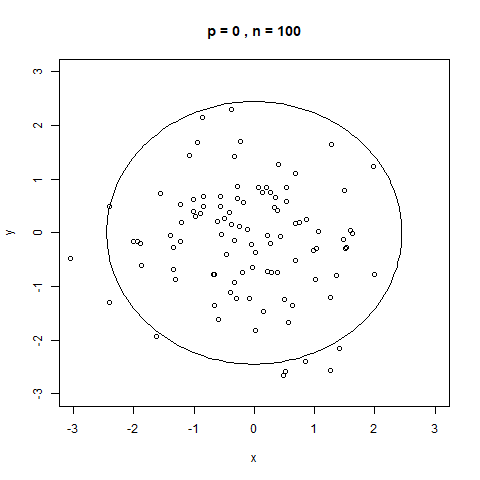
\includegraphics[width=0.3\textwidth]{100_0}
    \caption{$\rho=0, n=100$}
\end{figure}

\begin{figure}[!htb]
    \centering
    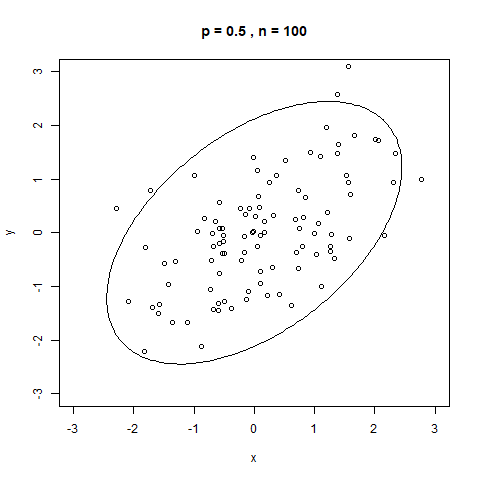
\includegraphics[width=0.3\textwidth]{100_0.5}
    \caption{$\rho=0.5, n=100$}
\end{figure}

\begin{figure}[!htb]
    \centering
    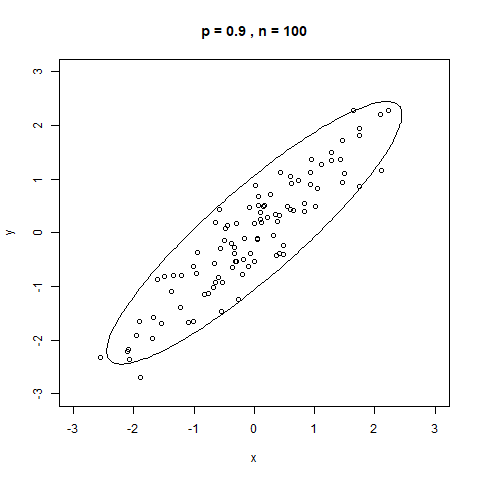
\includegraphics[width=0.3\textwidth]{100_0.9}
    \caption{$\rho=0.9, n=100$}
\end{figure}
\newpage
\subsection{Эллипсы рассеивания для выборки n=3}
\begin{figure}[!htb]
    \centering
    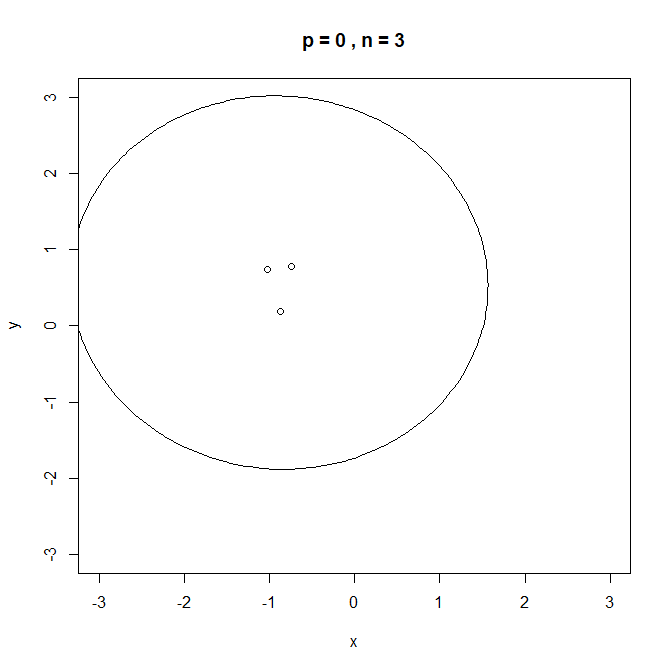
\includegraphics[width=0.3\textwidth]{plot_1}
    \caption{$\rho=0, n=3$}
\end{figure}

\begin{figure}[!htb]
    \centering
    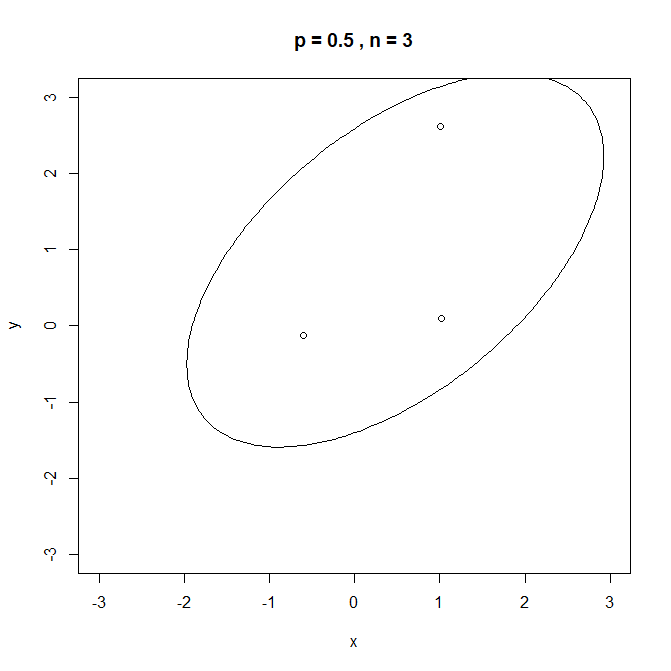
\includegraphics[width=0.3\textwidth]{plot_2}
    \caption{$\rho=0.5, n=3$}
\end{figure}

\begin{figure}[!htb]
    \centering
    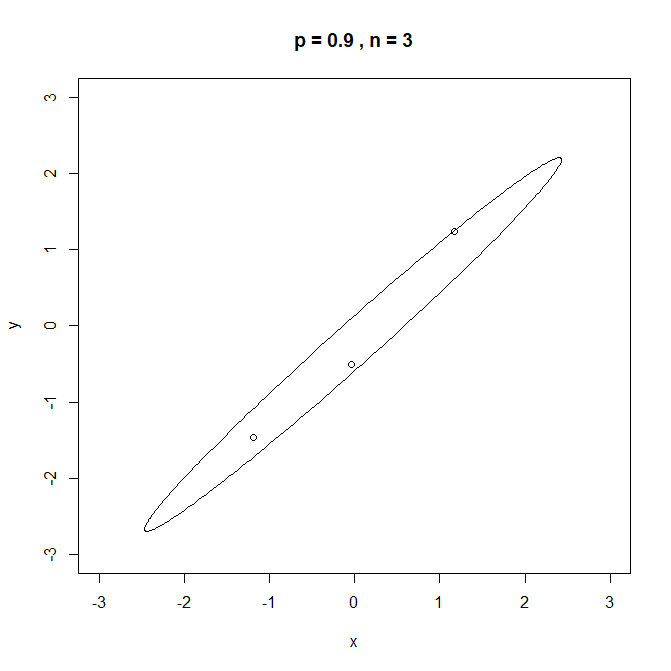
\includegraphics[width=0.3\textwidth]{plot_3}
    \caption{$\rho=0.9, n=3$}
\end{figure}
\newpage
\section{Обсуждение}
Сравним дисперсии выборочных коэффициентов корреляции.\\
Для двумерного нормального распределения дисперсии выборочных коэффициентов корреляции упорядочены следующим образом: $r<r_S<r_Q$.\\
Для смеси нормальных распределений дисперсии выборочных коэффициентов корреляции упорядочены следующим образом: $r<r_S<r_Q$.\\
Процент попавших элементов выборки в эллипс рассеивания (95\%-ная доверительная область) примерно равен его теоретическому значению (95\%).

\section{Приложения}
Репозиторий на Github с кодом лабораторной работы:\\
\url{https://github.com/VsevolodMelnikov/Math_Stat/tree/master/lab4}

\end{document}